\newpage
\appendix
%\addappheadtotoc
\addcontentsline{toc}{chapter}{Приложение}
\chapter{Скриншоты разрабатываемого приложения}\label{ap:screenshot}

\begin{figure}[h!] 
\centering 
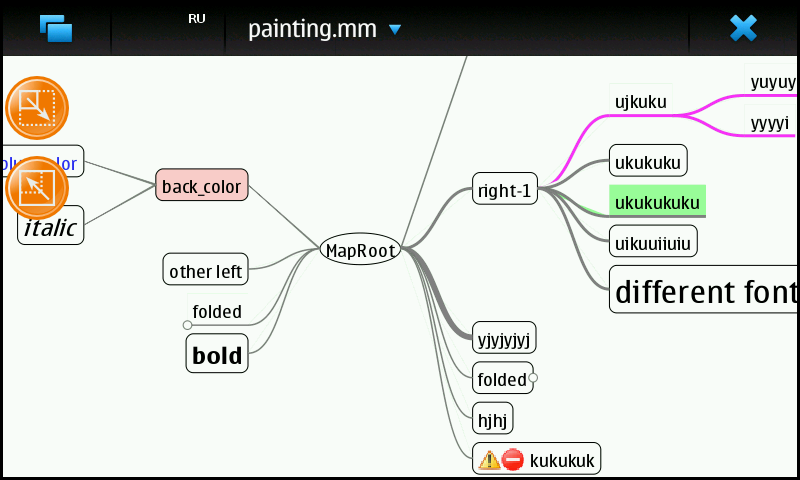
\includegraphics[width=1\linewidth]{main_view} 
\caption{Отображение модели диаграммы связей}
\label{ris:main_view}
\end{figure}

\begin{figure}[h!] 
\centering 
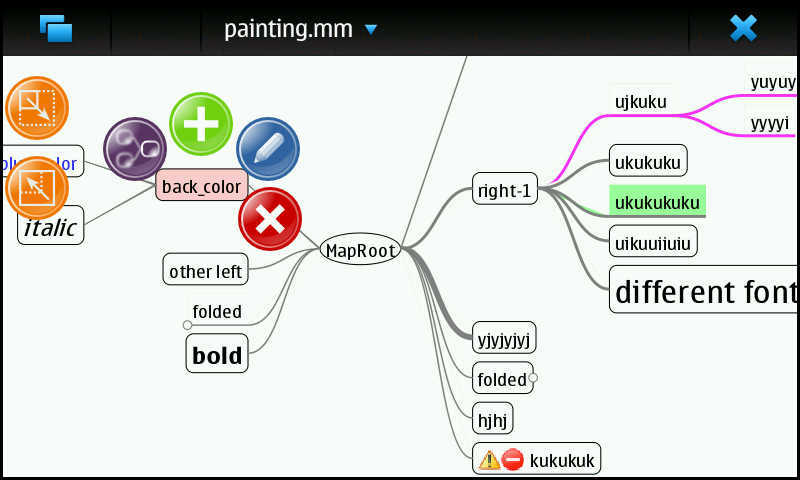
\includegraphics[width=0.6\linewidth]{context_menu} 
\caption{Контекстное меню узла}
\label{ris:context_menu}
\end{figure}

\begin{figure}[h!]
\begin{minipage}[h]{0.45\linewidth}
\center{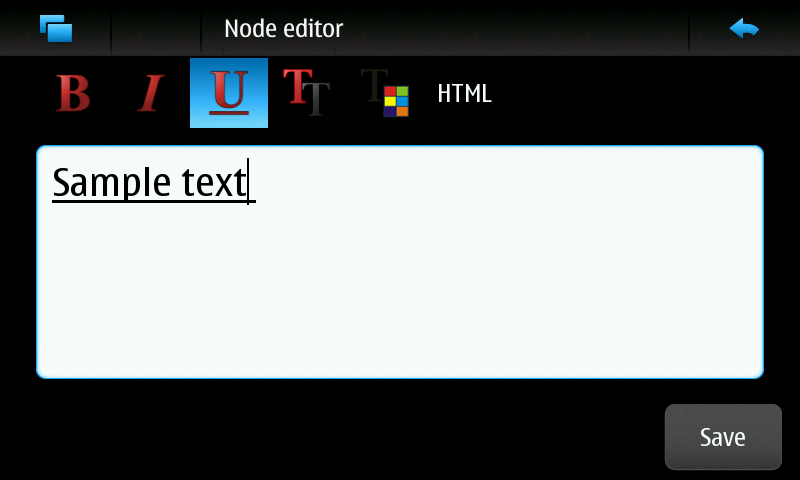
\includegraphics[width=1\linewidth]{text_dialog}} a) Главное окно редактора\\
\end{minipage}
\hfill
\begin{minipage}[h]{0.45\linewidth}
\center{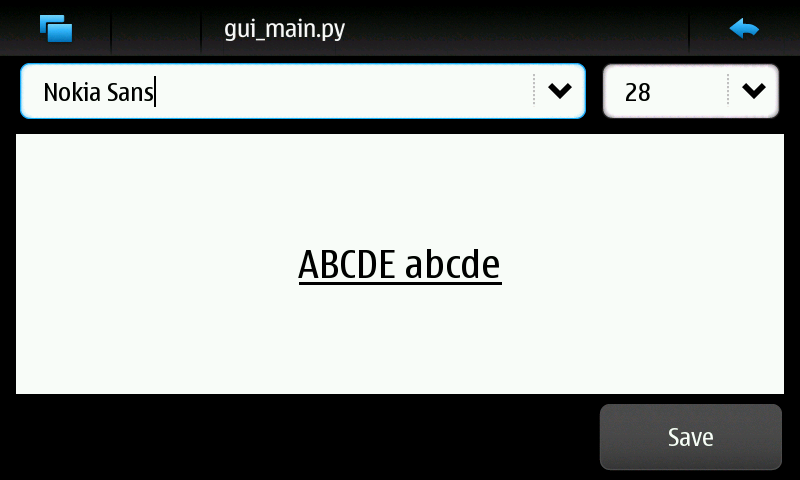
\includegraphics[width=1\linewidth]{font_dialog}} b) Диалог выбора шрифта\\
\label{ris:font_dialog}
\end{minipage}
\vfill
\begin{minipage}[h]{0.45\linewidth}
\center{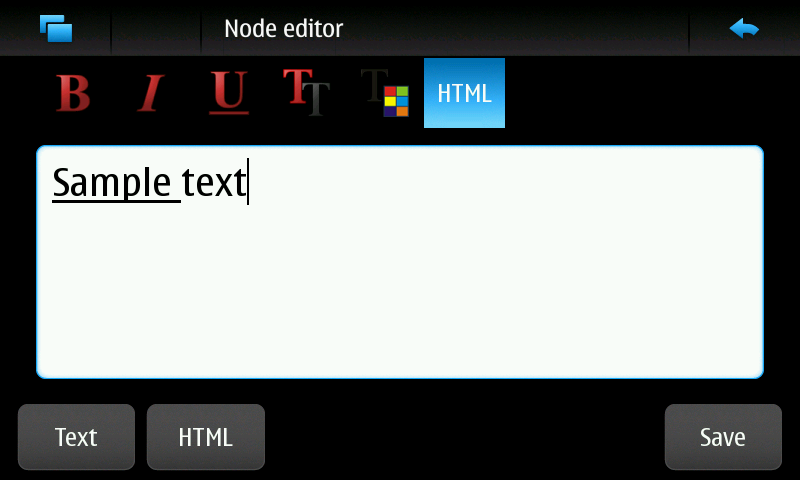
\includegraphics[width=1\linewidth]{html_editor}} c) Режим редактирования HTML\\
\end{minipage}
\hfill
\begin{minipage}[h]{0.45\linewidth}
\center{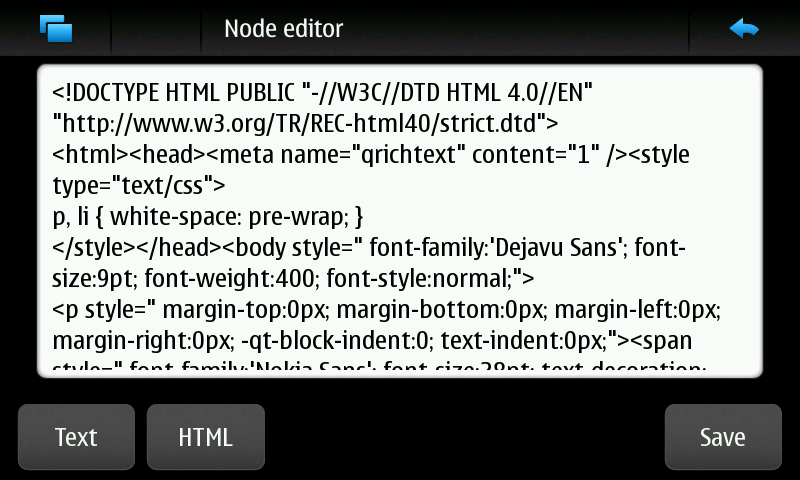
\includegraphics[width=1\linewidth]{html_source}} d) Редактирование исходного кода HTML\\
\end{minipage}
\caption{Редактор текста}
\label{ris:text_editor}
\end{figure}

\begin{figure}[h!] 
\centering 
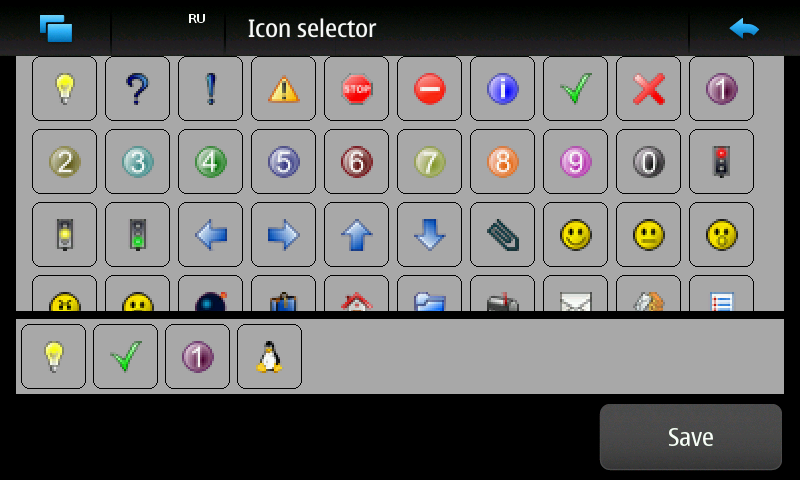
\includegraphics[width=1\linewidth]{icon_selector} 
\caption{Диалог выбора иконок}
\label{ris:icons_selector}
\end{figure}
\chapter{Диаграмма взаимодействия модели и вида}\label{ap:uml_scene}

\begin{figure}[h!] 
\centering 
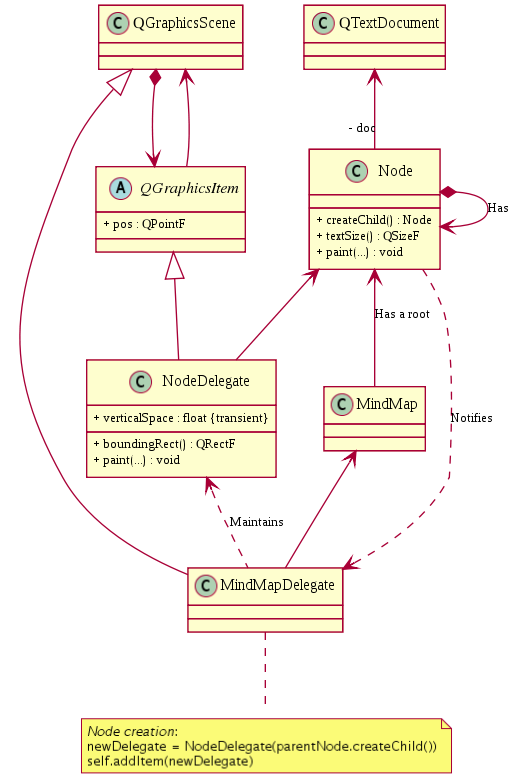
\includegraphics[width=0.5\linewidth]{uml_graphics} 
\caption{Диаграмма взаимодействия модель-вид}
\label{ris:uml_scene}
\end{figure}